% ===================================================================== B ====
\section{Proofs and exact numerics}
\label{app:proofs}

Write $H_Q(d)=\operatorname{rank}(\mathrm{Res}_Q|_{\mathcal P_{\le d}})$ for the \emph{Hilbert profile}, the number of independent
constraints the evidence imposes. On an affine slice, recompute and clamped patching can constrain equally many
alternatives while missing different ones.
\begin{proposition}[Equal Hilbert profile, different blind spaces]
\label{prop:incomparable}
On the affine two-site slice with $e(a)=ma+c$ and $b_0=ma_0+c$, let $N_R$ and $N_C$ be the degree-$d$ blind spaces
of the recompute and clamped single-site families. (i) $H_{Q_R}(d)=H_{Q_C}(d)=2d+1$ for every $d$. (ii) If $m\neq0$
and $d\ge2$, then $N_R\not\subseteq N_C$ and $N_C\not\subseteq N_R$. (iii) If $m\neq0$, then $N_R\cap N_C=h\cdot
\mathcal P_{\le d-3}$ with $h=(a-a_0)(b-ma-c)(b-b_0)$, of dimension $(d-1)(d-2)/2$ for $d\ge3$ and $0$ for $d<3$.
\end{proposition}

Counts alone cannot rank these two \emph{single-site} designs on an exact slice; the proposition says nothing about
single-site versus joint evidence in a trained model. Given $b_0=ma_0+c$, the submitted condition
$(m,c)\neq(0,b_0)$ is equivalent to $m\neq0$.

\emph{Proof.} (i) Count the constraints. Each reachable set comprises two lines, whose vanishing polynomials are
multiples of a degree-2 generator $g$. Thus $N=g\cdot\mathcal P_{\le d-2}$ has dimension $d(d-1)/2$ and profile
$\binom{d+2}{2}-d(d-1)/2=2d+1$.

(ii) Each generator witnesses incomparability. For $d\ge2$, $g_R\in N_R$ but $g_R\notin N_C$ because
$(b-b_0)\nmid(b-ma-c)$ when $m\neq0$; symmetrically $g_C\in N_C\setminus N_R$. For $d\le1$ both spaces are zero.

(iii) Find the shared blind differences. $p\in N_R\cap N_C$ iff $p=g_Ru=g_Cv$; cancelling $(a-a_0)$ gives
$(b-ma-c)u=(b-b_0)v$. The linear forms are non-associate when $m\neq0$. Unique factorisation in $\mathbb R[a,b]$
then gives $(b-b_0)\mid u$ and $p\in\langle h\rangle$; conversely, multiples of $h$ of degree at most $d$ lie in both spaces.
Equivalently, $N_R\cap N_C$ is generated by $\mathrm{lcm}(g_R,g_C)$ \citep{pistone1996groebner}. $\square$

\paragraph{Theorem~\ref{thm:operator}.} Find the vanishing polynomials on each arm, then intersect.
$I(A_0)=(a-a_0)$ because $A_0$ is an infinite subset of the line $a=a_0$.
$P$ vanishes on $\Gamma$, so $(P)\subseteq I(\Gamma)$. Conversely, if $Q$ vanishes on $\Gamma$ and $P\nmid Q$, then $P$
and $Q$ are coprime because $P$ is irreducible, so by B\'ezout's theorem $V(P)\cap V(Q)$ is finite, contradicting
$\Gamma\subseteq V(P)\cap V(Q)$ with $\Gamma$ infinite. Hence $I(\Gamma)=(P)$. Since $P$ is not an associate of
$a-a_0$, the two irreducibles are coprime and $I(A_0\cup\Gamma)=(a-a_0)\cap(P)=((a-a_0)P)$, whose nonzero elements
have degree at least $1+\deg P$. $\square$

The submitted version assumed only that $\Gamma$ is Zariski-dense in an irreducible $V(P)$. Over $\mathbb R$ this does
not give $I(\Gamma)=(P)$: for $P=(b-ma-c)^2$ the zero set is the irreducible line $b=ma+c$, but $I(\Gamma)=(b-ma-c)$,
so the onset is $2$, not $1+\deg P=3$. The affine and nondegenerate normalisation instances satisfy the corrected
hypothesis, so their onsets are unchanged. The transcendental instances are covered by the separate lemma below,
and their infinite onsets are also unchanged.

\paragraph{Irreducibility of the normalisation quartic.} To apply the operator theorem, rule out lower-degree
factors. Clearing the radical in
$e(a)=\beta+\omega a/\sqrt{\kappa a^2+\epsilon}$ gives $P(a,b)=(b-\beta)^2(\kappa a^2+\epsilon)-\omega^2a^2$, under
$\omega\neq0$, $\kappa>0$ and $\epsilon>0$ (for RMSNorm, $\epsilon$ is the model dimension times the normalisation
constant). As a quadratic in $X=b-\beta$ over $\mathbb R[a]$ it is $(\kappa a^2+\epsilon)X^2-\omega^2a^2$, with
discriminant $4\omega^2a^2(\kappa a^2+\epsilon)$. It factors over $\mathbb R[a]$ only if $\kappa a^2+\epsilon$ is a
square, which it is not, since it has two distinct complex roots; a factorisation with a factor free of $X$ would
need a common factor of $\kappa a^2+\epsilon$ and $\omega^2a^2$, and there is none. Hence $P$ is irreducible of degree
$4$ and not an associate of $a-a_0$, and the recompute branch is an infinite subset of $V(P)$, so
Theorem~\ref{thm:operator} gives $d^*=\DstarRMSNorm$.

\paragraph{Transcendence of the analysed slices.}
The following lemma rules out exact polynomial blind differences on the stated softmax and gated slices.
\begin{lemma}
Let $e(a)=\omega\,\sigma(ga)$ with $\sigma(x)=(1+\exp(-x))^{-1}$ and real $\omega,g\neq0$. No nonzero $P\in\mathbb
R[a,b]$ satisfies $P(a,e(a))\equiv0$ on an interval with nonempty interior.
\end{lemma}
\emph{Proof.} A polynomial relation for the sigmoid would imply one for the exponential.
Suppose $P(a,e(a))\equiv0$ with $P\neq0$. Then $e$ is algebraic over $\mathbb R(a)$: it satisfies a polynomial
equation with rational-function coefficients. Since $e=\omega/(1+\exp(-ga))$, the rational expression
$E:=\exp(-ga)=\omega/e-1$ is also algebraic over $\mathbb R(a)$. Clearing denominators gives
$\sum_{j=0}^np_j(a)\exp(-jga)=0$ with $p_j\in\mathbb R[a]$; divide out any power of $E$ to take $p_0\neq0$.
This expression is real analytic, so vanishing on an interval with nonempty interior implies vanishing identically.
Now let $a\to+\infty$ if $g>0$, or $a\to-\infty$ if $g<0$. Terms with $j\ge1$ decay exponentially while $p_j$
grows at most polynomially, forcing $p_0(a)\to0$, impossible for a nonzero polynomial. $\square$

A two-key softmax edge $e(a)=\omega\exp(a)/(\exp(a)+\exp(\kappa))=\omega\,\sigma(a-\kappa)$ with $\omega\neq0$ has the
lemma's form after a shift, so $I(\Gamma)=(0)$ and $d^*=\infty$ on that slice. For a gated linear-attention edge
$e(a)=(wa)\,\sigma(ga)$ with $w,g\neq0$, a relation $P(a,e(a))\equiv0$ would make $\sigma(ga)=e/(wa)$ algebraic over
$\mathbb R(a)$ on a subinterval with nonempty interior avoiding $a=0$, and the lemma applies again. Both statements concern the analysed slice
in the chosen coordinates (Remark~\ref{rem:scope}).

\paragraph{Proposition~\ref{prop:ksite}.} On arm $i$ the swept coordinate $t$ parameterises the arm, and every
coordinate is a polynomial in $t$ of degree at most $\eta_i$ (a constant has degree $0\le\eta_i$). Restricting a
degree-$d$ hypothesis gives a univariate polynomial of degree at most $d\eta_i$, hence at most $d\eta_i+1$
independent constraints. The $k$ arms agree at the clean configuration, imposing $k-1$ constraints and reducing
$\sum_i(d\eta_i+1)$ to $1+d\sum_i\eta_i$. Subtracting the restriction rank from the class dimension gives the bound.

The degrees must include all downstream compositions: with edges $A\to B\to C$ of degree $p$, patching $A$ leaves $b$ of degree
$p$ but $c$ of degree $p^2$. On a chain with $k=\KCEk$ sites, edge degree $\KCEe$ and $d=\KCEd$, using the edge degree
for every arm gives $\KCEBound$, whereas the exact rank (over a finite field, generic coefficients, edges shared across
arms) is $\KCERankExact$; the composed bound, $\KCEComposedBound$, holds.

\emph{Affine arms attain the bound.} Translate the clean state to the origin. Under the feed-forward order of
the sites, the arm directions form a triangular matrix with unit diagonal, so an invertible linear map sends the
arms to the coordinate axes. On the axes, the restrictions of $1$ and $x_i^r$ ($1\le i\le k$, $1\le r\le d$) are
linearly independent, so the rank is exactly $1+kd$. A Cartesian product with at least $d+1$ distinct values per axis
determines every polynomial of degree at most $d$ in each variable, so for $d=3$ four values per axis suffice. At degree $3$, single-site evidence then leaves unresolved $\KBlindTwo\%$ of the
class at two sites, $\KBlindThree\%$ at three, $\KBlindFour\%$ at four and $\KBlindFive\%$ at five.

\paragraph{Numerical checks of the exact results.} The left panel of Figure~\ref{fig:regimes} corroborates the
operator-slice results. On each of three sampling spans, singular value decomposition (SVD) fits a candidate
polynomial, the right singular vector for the smallest singular value of the column-scaled design. Its relative
residual reaches numerical precision at $d^*$ on the affine and RMSNorm slices, while the plotted softmax residual
decreases over the tested degrees. Numerics cannot certify that no polynomial relation exists; for the
transcendental slices the proof is the lemma above.

% ===================================================================== C ====
\section{Glossary}
\label{app:glossary}

\begin{center}\small
\begin{tabularx}{\textwidth}{@{}l>{\raggedright\arraybackslash}X@{}}
\toprule
term & meaning \\
\midrule
chart & a map from the sites' outputs to low-dimensional coordinates $z=(a,b,\dots)$ \\
reachable set $R_Q$ & the chart states an intervention family produces \\
blind space $N(Q,\mathcal F)$ & hypothesis differences in the class $\mathcal F$ that vanish on all of $R_Q$ \\
resolving preorder $\succeq_{\mathcal F}$ & $Q_1\succeq_{\mathcal F}Q_2$ when $N(Q_1,\mathcal F)\subseteq N(Q_2,\mathcal F)$: $Q_1$ resolves at least what $Q_2$ resolves \\
onset $d^*$ & the least polynomial degree at which the blind space is nonzero \\
recompute / clamped generator & on an affine slice, the degree-2 generators of the respective single-site blind spaces: $g_R=(a-a_0)(b-ma-c)$ and $g_C=(a-a_0)(b-b_0)$ \\
energy $E_Q(h)$ & mean square of a hypothesis difference over the family's states, $\theta^\top G_Q\theta$ \\
held-out $J/S$ energy ratio $r(h)$ & $E_J(h)/E_S(h)$ on test rows, for $h$ defined from training rows only \\
S-weak & a direction with a large $r(h)$: much less constrained by single-site than joint evidence \\
edge strength $s$ & $\mathrm{sd}(b\mid\text{arm }A)/\mathrm{sd}(b\mid\text{arm }B)$ strong if $s\ge0.10$; computed on training single-site rows for the named direction, and on all single-site rows in the support-matching and IOI analyses \\
same-family envelope & the null band for optimised directions built by splitting the single-site family (\S\ref{sec:practical}) \\
capture, cell, head pair & a capture is one (site pair, seed) run; a cell is a model $\times$ task. In \S\ref{sec:ioi}, a head pair is a (source head, Name Mover) pair, and a capture is that pair with a prompt \\
transport contrast $T_C$ & how much $B$'s measured effect changes when $A$ moves from its clean output to $u$: the four-point contrast $Y(u,v)-Y(u,0)-Y(0,v)+Y(0,0)$ of \S\ref{sec:ioi} \\
B-arm swing & the range of the readout over the single-site $B$ arm; the denominator of every ``\% of swing'' \\
working-model identification width & at a joint state, the largest $|T_C|$ inside a fit's nominal $95\%$ Wald region under the working model; summarised by a median over joint states within each capture, then a median over captures; neither an observed error nor a calibrated bound \\
design gap & the ratio, joint over single-site, of the smallest eigenvalue of the per-observation residualised design Gram of the cross block \\
\bottomrule
\end{tabularx}
\end{center}

% ===================================================================== D ====
\section{Protocol}
\label{app:protocol}

\paragraph{Protocol at a glance.} The following protocol underlies Sections~\ref{sec:practical} to~\ref{sec:pitfalls}; support and chart variants are
specified with each comparison.
\begin{itemize}[leftmargin=1.2em,itemsep=1pt,topsep=1pt,parsep=0pt]
\item \textbf{Units.} A \emph{capture} is one (site pair, seed) run, the seed selecting prompt and donors; a
\emph{cell} is a model $\times$ task. Table~\ref{tab:predict} has $\MatchedN$ float32 captures in $\PredCells$ cells and
$\HeldoutPrompts$ (cell, prompt) groups. Captures share models, tasks and often prompts, so counts are consistency
checks, and we make no population claim.
\item \textbf{Sites and chart.} Two attention-block outputs, each projected on the unembedding difference of the
task's two answer tokens, then whitened with statistics from training rows (the archived optimised profiles use
all-row statistics, which is equivalent in exact arithmetic; see below). The head-level IOI analysis of
\S\ref{sec:ioi} uses a different chart.
\item \textbf{Single-site family $S$.} $32$ donors $\times$ $\NAlpha$ interpolation coefficients $\alpha\in[-0.5,1.5]$
on each arm: patch $A$ and recompute $B$, or patch $B$ with $A$ clean. Each row is one intervention, giving $448$ rows.
\item \textbf{Joint family $J$.} $256$ rows on the same $\alpha$ grid, pairing donors and coefficients in a fixed
sparse pattern; it is not a full product grid.
\item \textbf{Class and split.} Polynomials of total degree at most $3$ ($10$ dimensions). Rows are split in half
($S$: $224/224$; $J$: $128/128$); directions are named or fitted on training rows, frozen, and scored on test rows.
\item \textbf{Screen.} Captures with $\mathrm{sd}(Y_{\mathrm{joint}})<0.15$ are excluded. In
Sections~\ref{sec:practical} to~\ref{sec:pitfalls} this is the only use of readouts, and it makes the analysed sample
readout-conditioned.
\end{itemize}

\paragraph{Families.} Each capture patches two sites. A donor--coefficient pair sets a site's output to
$o_{\mathrm{clean}}+\alpha\,(o_{\mathrm{donor}}-o_{\mathrm{clean}})$, where $o_{\mathrm{donor}}$ is the site's output on
the donor prompt. The single-site family has, for each of $32$ donors and each
of the $\NAlpha$ coefficients $\alpha\in\{-0.5,-\tfrac16,\tfrac16,0.5,\tfrac56,\tfrac76,1.5\}$, one row patching $A$
with $B$ recomputed and one row patching $B$ with $A$ clean: $448$ rows. The support-matched joint family has $256$
rows. Row $r=16i+j$ ($i,j\in\{0,\dots,15\}$) pairs donors $2i$ and $2j$ with the coefficient indices $(i+j)\bmod 7$
and $(3i+j)\bmod 7$; on each axis it uses $112$ of the $224$ single-site (donor, coefficient) pairs, a sparse subset
of their Cartesian product. The query-chart captures of \S\ref{sec:ioi} index donors by donor id instead. Both joint
families of Appendix~\ref{app:matched} are collected in one pass with the single-site family, on identical prompts,
donors and weights.

\paragraph{Training statistics and archived profiles.} For the named direction, the edge fit, whitening and
column scaling use training rows only. The archived optimised
polynomial profiles (Figure~\ref{fig:regimes}, right, \S\ref{sec:pitfalls} and Appendices~\ref{app:matched},
\ref{app:chart} and~\ref{app:three}) estimate whitening and column scaling on all analysed rows. For a fixed chart
and the complete, degree-ordered monomial bases used there, changing to training-row statistics is an invertible
lower-triangular change of feature basis with positive diagonal. This leaves the Cholesky-reduced covariant
eigenproblem unchanged in exact arithmetic. On identical row partitions, the fitted eigenfunctions therefore agree
up to scale, and the held-out profiles and same-family envelopes are unchanged. Numerically this holds only where the
held-out energies are resolved: at the clamped-weak end of Appendix~\ref{app:chart} the clamped family has an exact
polynomial kernel, so those energies are at rounding level under either choice. This does not cover chart selection
itself or the Euclidean-ridge checks of Appendices~\ref{app:robust} and~\ref{app:noninvariant}.

\paragraph{Precision.} All support-matched captures behind Table~\ref{tab:predict} and all IOI query-chart captures
are float32. The earlier unmatched captures of GPT-2 on IOI and of Qwen3.5-9B-Base were produced with a bfloat16
model, so their recorded states as well as their readouts carry bfloat16 rounding; the other GPT-2 unmatched captures
are float32. Comparisons with those earlier captures therefore also change precision.

\paragraph{Readout screen.} A capture is analysed only if $\mathrm{sd}(Y_{\mathrm{joint}})\ge0.15$. No readout enters
the naming or scoring of a direction, but the analysed sample is conditioned on the readout through this screen.
In the IOI query-chart analysis, $36$ published and $36$ control captures were designed and $\QCN$ and $\QCCtrlN$ kept;
the collector dropped captures that failed the screen or raised an exception without recording which.

\paragraph{Same-family envelope.} For optimised directions we compare the held-out profile with a same-family envelope.
We split $S$ into two stand-in families and run the identical train--freeze--score procedure. Within each cell, we
pool the other captures' null profiles and take the $2.5$th percentile of their minima and the $97.5$th percentile
of their maxima, leaving each capture's own nulls out. In the full-grid single-site--joint comparison, each stand-in
family has $112$ training and $112$ test rows, against $224/224$ for $S$ and $128/128$ for $J$. These sample sizes differ,
and captures share prompts, so the nominal $2.5\%$ escape rate is not established for the tested procedure. We report escape counts
descriptively and any $p$-values as nominal (Appendix~\ref{app:corrections}, C32).

\paragraph{Applying the audit to another circuit.} (1) Declare $\mathcal F$; the chosen polynomial degree limits which
hypothesis differences the audit can assess. (2) Sweep the intervention family and record the internal states, not just
the readout. (3) Form $G_Q$ and read off its low-energy directions; with a second family, solve the covariant
pencil. (4) Before comparing two families, check that their reachable sets span the same region; for optimised
directions, compare with a same-family envelope, remembering that its $p$-values are nominal. (5) For a transport
claim, execute the clamped and joint corners and measure the numerical floor by re-executing them in a different
batch composition. Only steps (2) and (5) need GPU time.

% ===================================================================== E ====
\section{Support matching in full}
\label{app:matched}

Two further protocols separate the effect of removing extrapolation from that of enlarging the joint family.
\emph{Interior} restricts the single-site family to $\alpha\in[0,1]$ and leaves the joint family at $\alpha=1$; it
needs no new data but is conservative rather than exact. \emph{Symmetric} restricts both families to the interior
coefficients, which answers the objection that matching helped only by enlarging the joint family. Across all
$\MatchedN$ support-matched captures the reverse end escapes the same-family envelope in $\EdgeFrozenEscapes$
captures under the unmatched protocol, $\EdgeInteriorEscapes$ under interior, $\EdgeSymmetricEscapes$ under symmetric
and $\EdgeMatchedEscapes$ under matched.

Edge strength is associated with a reverse escape under the matched (Spearman $\EdgeMatchedRho$), interior
($\EdgeInteriorRho$) and symmetric ($\EdgeSymmetricRho$) protocols, and only weakly under the unmatched one
($\EdgeFrozenRho$). Under the matched protocol the median edge strength is $\EdgeMatchedMedEscaped$ for escapes against
$\EdgeMatchedMedNot$ for non-escapes. These correlations, the edge-strength medians and survivor count of \S\ref{sec:pitfalls}, and
Figure~\ref{fig:matched} use the edge statistic stored with the matched analysis: the arm-$A$/arm-$B$ spread ratio
computed on all single-site rows rather than on training rows only; the paragraph on the realised edge below uses the
training-row statistic $s$ of \S\ref{sec:predict}. Figure~\ref{fig:spectrum} shows the held-out profiles behind
Table~\ref{tab:matched-full}, and Figure~\ref{fig:matched} the escape rates and their association with edge strength.
Table~\ref{tab:predict-unmatched} repeats the $g_R$ columns of Table~\ref{tab:predict} against the unmatched joint
family on the earlier unmatched captures.

\begin{table}[!htbp]
\centering\small
\begin{tabular}{llcccc}
\toprule
model $\times$ task & protocol & low end & $q$ & reverse end & $q$ \\
\midrule
\multirow{4}{*}{GPT-2 $\times$ IOI}
 & joint at $1$ & \MGPTIOIFrozenSblind & $\MGPTIOIFrozenQS$ & \MGPTIOIFrozenJblind & $\MGPTIOIFrozenQJ$ \\
 & interior & \MGPTIOIInteriorSblind & $\MGPTIOIInteriorQS$ & \MGPTIOIInteriorJblind & $\MGPTIOIInteriorQJ$ \\
 & symmetric & \MGPTIOISymmetricSblind & $\MGPTIOISymmetricQS$ & \MGPTIOISymmetricJblind & $\MGPTIOISymmetricQJ$ \\
 & \textbf{matched} & \MGPTIOIMatchedSblind & $\MGPTIOIMatchedQS$ & \MGPTIOIMatchedJblind & $\MGPTIOIMatchedQJ$ \\
\midrule
\multirow{4}{*}{GPT-2 $\times$ induction}
 & joint at $1$ & \MGPTIndFrozenSblind & $\MGPTIndFrozenQS$ & \MGPTIndFrozenJblind & $\MGPTIndFrozenQJ$ \\
 & interior & \MGPTIndInteriorSblind & $\MGPTIndInteriorQS$ & \MGPTIndInteriorJblind & $\MGPTIndInteriorQJ$ \\
 & symmetric & \MGPTIndSymmetricSblind & $\MGPTIndSymmetricQS$ & \MGPTIndSymmetricJblind & $\MGPTIndSymmetricQJ$ \\
 & \textbf{matched} & \MGPTIndMatchedSblind & $\MGPTIndMatchedQS$ & \MGPTIndMatchedJblind & $\MGPTIndMatchedQJ$ \\
\midrule
\multirow{4}{*}{GPT-2 $\times$ capital}
 & joint at $1$ & \MGPTCapFrozenSblind & $\MGPTCapFrozenQS$ & \MGPTCapFrozenJblind & $\MGPTCapFrozenQJ$ \\
 & interior & \MGPTCapInteriorSblind & $\MGPTCapInteriorQS$ & \MGPTCapInteriorJblind & $\MGPTCapInteriorQJ$ \\
 & symmetric & \MGPTCapSymmetricSblind & $\MGPTCapSymmetricQS$ & \MGPTCapSymmetricJblind & $\MGPTCapSymmetricQJ$ \\
 & \textbf{matched} & \MGPTCapMatchedSblind & $\MGPTCapMatchedQS$ & \MGPTCapMatchedJblind & $\MGPTCapMatchedQJ$ \\
\midrule
\multirow{4}{*}{GPT-2 $\times$ greater-than}
 & joint at $1$ & \MGPTGtFrozenSblind & $\MGPTGtFrozenQS$ & \MGPTGtFrozenJblind & $\MGPTGtFrozenQJ$ \\
 & interior & \MGPTGtInteriorSblind & $\MGPTGtInteriorQS$ & \MGPTGtInteriorJblind & $\MGPTGtInteriorQJ$ \\
 & symmetric & \MGPTGtSymmetricSblind & $\MGPTGtSymmetricQS$ & \MGPTGtSymmetricJblind & $\MGPTGtSymmetricQJ$ \\
 & \textbf{matched} & \MGPTGtMatchedSblind & $\MGPTGtMatchedQS$ & \MGPTGtMatchedJblind & $\MGPTGtMatchedQJ$ \\
\midrule
\multirow{4}{*}{GPT-2 $\times$ agreement}
 & joint at $1$ & \MGPTAgrFrozenSblind & $\MGPTAgrFrozenQS$ & \MGPTAgrFrozenJblind & $\MGPTAgrFrozenQJ$ \\
 & interior & \MGPTAgrInteriorSblind & $\MGPTAgrInteriorQS$ & \MGPTAgrInteriorJblind & $\MGPTAgrInteriorQJ$ \\
 & symmetric & \MGPTAgrSymmetricSblind & $\MGPTAgrSymmetricQS$ & \MGPTAgrSymmetricJblind & $\MGPTAgrSymmetricQJ$ \\
 & \textbf{matched} & \MGPTAgrMatchedSblind & $\MGPTAgrMatchedQS$ & \MGPTAgrMatchedJblind & $\MGPTAgrMatchedQJ$ \\
\midrule
\multirow{4}{*}{Qwen3.5-9B $\times$ IOI}
 & joint at $1$ & \MQwenIOIFrozenSblind & $\MQwenIOIFrozenQS$ & \MQwenIOIFrozenJblind & $\MQwenIOIFrozenQJ$ \\
 & interior & \MQwenIOIInteriorSblind & $\MQwenIOIInteriorQS$ & \MQwenIOIInteriorJblind & $\MQwenIOIInteriorQJ$ \\
 & symmetric & \MQwenIOISymmetricSblind & $\MQwenIOISymmetricQS$ & \MQwenIOISymmetricJblind & $\MQwenIOISymmetricQJ$ \\
 & \textbf{matched} & \MQwenIOIMatchedSblind & $\MQwenIOIMatchedQS$ & \MQwenIOIMatchedJblind & $\MQwenIOIMatchedQJ$ \\
\midrule
\multirow{4}{*}{Qwen3.5-9B $\times$ induction}
 & joint at $1$ & \MQwenIndFrozenSblind & $\MQwenIndFrozenQS$ & \MQwenIndFrozenJblind & $\MQwenIndFrozenQJ$ \\
 & interior & \MQwenIndInteriorSblind & $\MQwenIndInteriorQS$ & \MQwenIndInteriorJblind & $\MQwenIndInteriorQJ$ \\
 & symmetric & \MQwenIndSymmetricSblind & $\MQwenIndSymmetricQS$ & \MQwenIndSymmetricJblind & $\MQwenIndSymmetricQJ$ \\
 & \textbf{matched} & \MQwenIndMatchedSblind & $\MQwenIndMatchedQS$ & \MQwenIndMatchedJblind & $\MQwenIndMatchedQJ$ \\
\midrule
\multirow{4}{*}{Qwen3.5-9B $\times$ capital}
 & joint at $1$ & \MQwenCapFrozenSblind & $\MQwenCapFrozenQS$ & \MQwenCapFrozenJblind & $\MQwenCapFrozenQJ$ \\
 & interior & \MQwenCapInteriorSblind & $\MQwenCapInteriorQS$ & \MQwenCapInteriorJblind & $\MQwenCapInteriorQJ$ \\
 & symmetric & \MQwenCapSymmetricSblind & $\MQwenCapSymmetricQS$ & \MQwenCapSymmetricJblind & $\MQwenCapSymmetricQJ$ \\
 & \textbf{matched} & \MQwenCapMatchedSblind & $\MQwenCapMatchedQS$ & \MQwenCapMatchedJblind & $\MQwenCapMatchedQJ$ \\
\midrule
\multirow{4}{*}{Qwen3-8B $\times$ IOI}
 & joint at $1$ & \MQIOIFrozenSblind & $\MQIOIFrozenQS$ & \MQIOIFrozenJblind & $\MQIOIFrozenQJ$ \\
 & interior & \MQIOIInteriorSblind & $\MQIOIInteriorQS$ & \MQIOIInteriorJblind & $\MQIOIInteriorQJ$ \\
 & symmetric & \MQIOISymmetricSblind & $\MQIOISymmetricQS$ & \MQIOISymmetricJblind & $\MQIOISymmetricQJ$ \\
 & \textbf{matched} & \MQIOIMatchedSblind & $\MQIOIMatchedQS$ & \MQIOIMatchedJblind & $\MQIOIMatchedQJ$ \\
\midrule
\multirow{4}{*}{Qwen3-8B $\times$ induction}
 & joint at $1$ & \MQIndFrozenSblind & $\MQIndFrozenQS$ & \MQIndFrozenJblind & $\MQIndFrozenQJ$ \\
 & interior & \MQIndInteriorSblind & $\MQIndInteriorQS$ & \MQIndInteriorJblind & $\MQIndInteriorQJ$ \\
 & symmetric & \MQIndSymmetricSblind & $\MQIndSymmetricQS$ & \MQIndSymmetricJblind & $\MQIndSymmetricQJ$ \\
 & \textbf{matched} & \MQIndMatchedSblind & $\MQIndMatchedQS$ & \MQIndMatchedJblind & $\MQIndMatchedQJ$ \\
\bottomrule
\end{tabular}
\caption{Escapes of the same-family envelope by the optimised profile's low end and reverse end, by protocol, over
all $\MatchedN$ support-matched captures; denominators are the screened captures in each cell. $q$ is a
Holm-adjusted binomial $p$-value against the envelope's nominal $2.5\%$ escape rate, adjusted across cells for each
protocol and end; it is nominal (\S\ref{sec:practical}). Under the matched protocol no cell retains a nominally
significant reverse end; under the interior protocol GPT-2 $\times$ induction and Qwen3.5-9B $\times$ induction do,
and under the symmetric protocol GPT-2 $\times$ induction does.}
\label{tab:matched-full}
\end{table}

\begin{figure}[h]
\centering
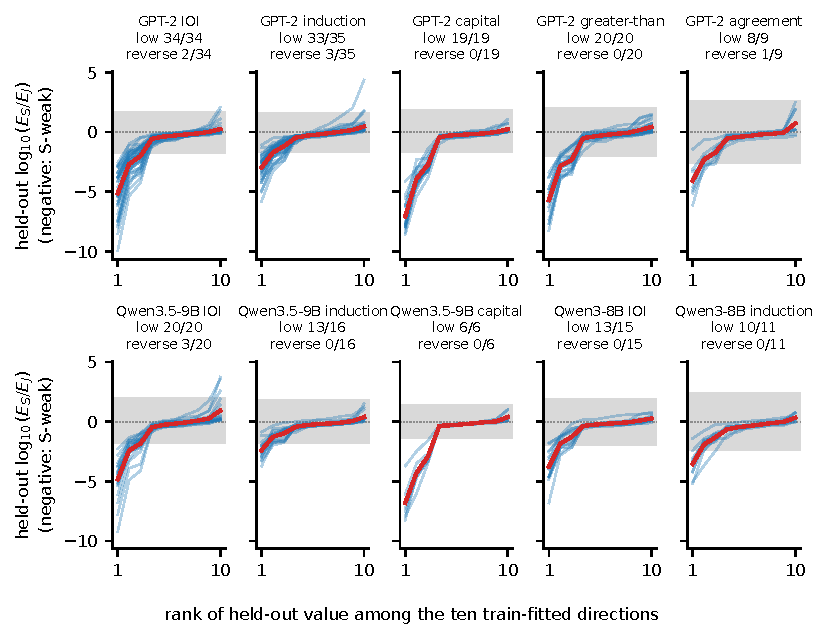
\includegraphics[width=\textwidth]{figures/fig_spectrum.pdf}
\caption{Held-out profiles behind Table~\ref{tab:matched-full}, support-matched protocol (joint family on the single-site $\alpha$ grid, a sparse design). For each capture (thin
blue lines) the ten generalized eigen-directions are fitted on training rows and frozen; the plot shows their held-out
$\log_{10}(E_S/E_J)$ energy ratios \emph{sorted by held-out value} (order statistics). Negative values are S-weak: single-site evidence constrains these hypothesis differences less than joint evidence does.
The low end is the minimum over the ten frozen directions, not the named generator of \S\ref{sec:predict}, and need
not be the first training eigenvector. The thick red line is the mean of the held-out order statistics. The grey band applies the percentiles of
Appendix~\ref{app:protocol} to the same-family nulls of all captures in the cell, pooled, and is shown for display; the
escape counts in the panel titles and in Table~\ref{tab:matched-full} leave each capture's own nulls out, as in
Appendix~\ref{app:protocol}. In GPT-2 $\times$ agreement, a reverse endpoint exceeds its leave-one-capture-out upper bound
while remaining below the displayed upper bound.}
\label{fig:spectrum}
\end{figure}

\begin{figure}[h]
\centering
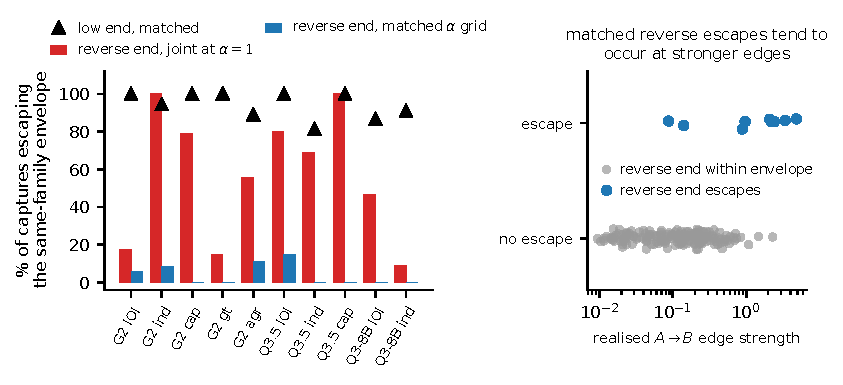
\includegraphics[width=\textwidth]{figures/fig_matched.pdf}
\caption{Support matching and escapes of the same-family envelope. \emph{Left:} percentages of captures whose
optimised profiles escape at the low (S-weak) or reverse (joint-weak) end: red bars, reverse end with the joint family at $\alpha=1$; blue bars, reverse end on
the matched grid; black triangles, low end on the matched grid. Matching reduces reverse escapes.
\emph{Right:} each point is a capture; edge strength (the matched analysis's all-rows statistic, logarithmic axis)
is plotted against the binary matched-protocol reverse-escape indicator, with vertical jitter. Blue points escape at the reverse end;
grey points do not escape at that end, although their low end may escape. Escapes are associated with stronger edges. Tick labels: G2, GPT-2; Q3.5, Qwen3.5-9B-Base; Q3-8B, Qwen3-8B;
ind, induction; cap, capital; gt, greater-than; agr, agreement.}
\label{fig:matched}
\end{figure}

\begin{table}[!htbp]
\centering\small
\begin{tabular}{lcc}
\toprule
model $\times$ task & median $r(g_R)$ & $r(g_R)>10\times$ \\
\midrule
GPT-2 $\times$ IOI          & $\PredGPTIOIRatio$  & \PredGPTIOICount \\
GPT-2 $\times$ induction    & $\PredIndGPTRatio$  & \PredIndGPTCount \\
GPT-2 $\times$ capital      & $\PredCapGPTRatio$  & \PredCapGPTCount \\
GPT-2 $\times$ greater-than & $\PredGtGPTRatio$   & \PredGtGPTCount \\
GPT-2 $\times$ agreement    & $\PredAgrGPTRatio$  & \PredAgrGPTCount \\
Qwen3.5-9B $\times$ IOI     & $\PredQwenIOIRatio$ & \PredQwenIOICount \\
Qwen3.5-9B $\times$ induction & $\PredIndQwenRatio$ & \PredIndQwenCount \\
Qwen3.5-9B $\times$ capital & $\PredCapQwenRatio$ & \PredCapQwenCount \\
\midrule
all                         &                     & \PredTotalCount \\
\bottomrule
\end{tabular}
\caption{Held-out $J/S$ energy ratios of the named generator $g_R$ against the unmatched joint family (raw donors,
$\alpha=1$), repeating its columns of Table~\ref{tab:predict} on the earlier unmatched captures. The qualitative result persists ($\PredTotalCount$ above $10\times$); the magnitude of the $J/S$
ratio depends on the joint support, and the cohorts differ in precision by cell (Appendix~\ref{app:protocol}).}
\label{tab:predict-unmatched}
\end{table}

\paragraph{The named generator and the one-at-a-time baseline.} In the captures, writing $b=ma+c+\varepsilon$ with the recorded
clean $b_0$, the clamped generator equals $m(a-a_0)^2+(a-a_0)(ma_0+c-b_0+\varepsilon)$. Both generators clear $10\times$ in
$\OfatBoth$ captures, $g_R$ alone in $\OfatOnlyRecompute$, $g_C$ alone in $\OfatOnlyClampedCount$, and neither in
$\OfatNeither$, a net difference of $\OfatNetDifference$. The median $r(g_R)$ is $\EdgeBlindWeak$ on weak-edge captures and
$\EdgeBlindStrong$ on the $\EdgeNStrong$ strong-edge ones, of which $\EdgeStrongGtTen$ exceed $10\times$. Of the surviving reverse
escapes of \S\ref{sec:pitfalls}, $\ReverseSurvivorsWeak$ fall below the strong-edge threshold. For the GPT-2 IOI captures, the
single-site range of $a$ exceeds its range under the unmatched joint family by a median factor of $\FigOneBCaptureMedian$,
the support gap behind Figure~\ref{fig:reachable}.

\paragraph{The realised edge, measured.} On all $\EdgeN$ support-matched captures, the absolute Euclidean cosine between the
recompute and clamped generators, in the fixed whitened, column-scaled coefficient basis, falls as the training-row edge strength
$s$ defined in \S\ref{sec:predict} rises (Spearman $\EdgeCosRho$; with the absolute whitened slope it is $\EdgeCosRhoSlope$). Its median is
$\EdgeWeakCos$ below $s=0.10$ and $\EdgeStrongCos$ on the $\EdgeNStrong$ captures at or above it. These cosines are
parameterisation-dependent and descriptive; they do not show that the two designs are equivalent. On the
strong-edge captures the median held-out ratio is $\EdgeStrongSepGC$ for $g_C$ and $\EdgeBlindStrong$ for $g_R$, and
the median within-capture ratio $r(g_R)/r(g_C)$ is $\EdgeStrongRatio$. The design comparison rests on these energy
ratios and on Table~\ref{tab:predict}: the one-at-a-time generator accounts for most threshold exceedances in this
chart, and the recompute generator has an additional advantage on stronger edges.

% ===================================================================== F ====
\clearpage
\section{Chart selection in full}
\label{app:chart}

This experiment compares recompute single-site evidence $R$ with clamped single-site evidence $C$, not single-site
with joint evidence. In the unembedding chart the absolute whitened edge slope is small (median $\RCUchartChartM$), so the
two designs almost coincide and both ends of their optimised profiles are nominally significant in only
$\RCUchartMutual$ cells. We therefore chose the
downstream coordinate by maximising a regularised variance ratio between the arms, using states only; the corresponding
spread ratio is $\mathrm{sd}(b\mid\text{arm }A)/\mathrm{sd}(b\mid\text{arm }B)$. In that chart the edge is strong (median $|m|=\RCChartM$). Scoring the held-out $R/C$ energy profile of the
train-fitted generalized eigen-directions, the recompute-weak end escapes the same-family envelope in $\RCPooledR$
captures, and the clamped-weak end escapes in every retained capture; both ends are nominally significant in
$\RCMutual$ cells.

The chart was fitted on states of the capture on which it was scored. In addition to the readout screen,
this analysis excludes captures with an arm-$A$/arm-$B$ spread ratio above $50$: $\RCDropped$ captures in the
own-chart and donor-holdout analyses. Holding out donors is not enough, because the chart is still fitted on the
capture's own prompt; the recompute-weak end still escapes in $\RCHoldoutPooledR$ captures.

With the chart of a different seed of the same layer pair, the
recompute-weak end escapes in $\RCXseedPooledR$ captures and both ends are nominally significant in $\RCXseedMutual$
cells (GPT-2 capital, GPT-2 IOI and Qwen3.5-9B capital). The cross-seed analysis covers the eight cells with an
available source chart, and its artifact predates the Qwen3-8B cross-seed captures, so the cohorts differ and the
comparison is not a paired effect estimate. For example, GPT-2 induction falls from $\RCGPTIndRblind$ to
$\RCGPTIndXseedRblind$.

A seed change does not partition content either:
$\AuditXseedSamePrompt$ evaluated captures share the chart source's base prompt, and donors are drawn from a shared
pool without a cross-seed exclusion rule. This is a cross-seed transfer control, not a disjoint-content
validation. The reversal between cells under this control is consistent with selection; the differing cohorts limit its interpretation.

The selection criterion is a variance ratio whose denominator is estimated from at most $16$ donor directions in a
much larger space ($768$ dimensions for GPT-2). In the GPT-2 captures for which this was logged, the selected direction had
negligible projection onto the span of the donor directions used to estimate the denominator, so its variance ratio was controlled by the
regulariser. The chart is therefore not ``the direction in which $A$ drives $B$'' but ``the direction in which $A$
drives $B$ and these particular donors do not''.

% ===================================================================== G ====
\section{Two planned hypotheses that failed, and two withdrawn claims}
\label{app:negatives}

Four planned hypotheses did not survive. Two are the withdrawn claims of \S\ref{sec:pitfalls}: (1) mutual
non-domination of single-site and joint evidence (support confound; Appendix~\ref{app:matched}) and (2) mutual
non-domination of recompute and clamped single-site evidence in a chart optimised on the scored states (chart
selection; Appendix~\ref{app:chart}). The other two failed their
criteria. Hypotheses (3) and (4) have dated preregistration records; for (1), registration and results first
enter version control together, so their order cannot be verified; for (2), no dated preregistration entry exists.

\paragraph{(3) Failed hypothesis: a circuit with high in-family faithfulness degrades reciprocally across families.} We fitted and froze
an edge-attribution circuit under each intervention family and scored it under both. The registered gate required
in-family faithfulness of at least $0.85$ and a cross-family drop of at least $0.25$ in both directions. It failed.
The recovered component sets largely overlapped, but overlap alone does not show that transfer cannot degrade. A
circuit is a set of components, whereas the ambiguity studied here lives in functional form, which a set cannot
express.

\paragraph{(4) Failed hypothesis: interpretability representations have distinctive weakly constrained subspaces.} We expected a logit
lens or a tuned lens to show S-weak subspaces distinguishable from matched compression controls. The registered success criterion required an effect outside the matched same-family and
compression nulls, a nontrivial held-out effect, and a consistent direction across multiple model-by-task units.
For $12$ GPT-2 captures in a four-dimensional chart, entries below are capture medians of the held-out energy share
$v_S=E_S/(E_S+E_J)$ of the least-energy training direction. The same-family null is rebuilt at each degree; each null
entry is the capture median of the per-capture $5$th percentile over five same-family resamples at the degree
indicated by its column header.

The arm we call the attention-output unembedding (the row the accepted version labelled ``logit lens''; C57) maps each
last-token attention-module output $A$ to $\rho(A)=\bigl((A-\bar A)/(\operatorname{sd}(A)+10^{-6})\bigr)W_U^{\top}$,
evaluated through its isometric SVD reduction; it uses this custom standardization rather than the model's learned final
LayerNorm and acts on attention outputs, not residual-stream states, so it is not the conventional logit lens. The arm
labelled ``tuned lens'' in the accepted version is a least-squares linear surrogate fitted to this attention-output
unembedding of the first capture's patch-$A$-arm rows and reused across captures and
sites. Of its calibration rows, $\TLCalibOverlap$ fall in that capture's scored half; only the subsequent chart
fit is restricted to training rows.

\begin{center}\small
\begin{tabular}{lrrrr}
\toprule
 & \multicolumn{2}{c}{share $v_S$} & \multicolumn{2}{c}{same-family null ($5$th pct.)} \\
\cmidrule(lr){2-3}\cmidrule(lr){4-5}
representation & $\mathcal F=\mathcal P_{\le1}$ & $\mathcal F=\mathcal P_{\le2}$ & $\mathcal F=\mathcal P_{\le1}$ & $\mathcal F=\mathcal P_{\le2}$ \\
\midrule
raw activations & $\MCRawDegOne$ & $\MCRawDegTwo$ & $\MCRawNull$ & $\MCRawNullTwo$ \\
attention-output unembedding & $\MCLLDegOne$  & $\MCLLDegTwo$  & $\MCLLNull$ & $\MCLLNullTwo$ \\
linear surrogate of it & $\MCTLDegOne$  & $\MCTLDegTwo$  & $\MCTLNull$ & $\MCTLNullTwo$ \\
\midrule
random projection (matched control) & $\MCRandDegOne$ & $\MCRandDegTwo$ & $\MCRandNull$ & $\MCRandNullTwo$ \\
\bottomrule
\end{tabular}
\end{center}

\noindent At degree $1$ each row's capture-median share lies below its degree-1 null by a factor of
$\MCNullRatioOneLo$--$\MCNullRatioOneHi$; at degree $2$ it lies below its degree-2 null by a factor of
$\MCNullRatioTwoLo$--$\MCNullRatioTwoHi$. These factors are ratios of the capture-median null to the capture-median
share, not medians of within-capture ratios. Degree-3 values fall below the numerical resolution of the computation,
where even an orthogonal reparameterisation moves them substantially, so we do not report them.

The captures cover one model-by-task unit (GPT-2, IOI). The compression control is one fixed pair of random site projections reused across
captures rather than a distribution over projections. The captures therefore cannot establish the criterion, which
was not met; this shows neither that representation effects are absent nor that any representation separates. At degree $2$
the attention-output-unembedding share is below the random-projection share in $\MCLLBelowRandTwo$ captures, the raw-activation share in
$\MCRawBelowRandTwo$ and the surrogate's share in $\MCTLBelowRandTwo$; the direction is therefore not specific to the
attention-output unembedding, and these are descriptive comparisons within that one unit. The registration treats cross-representation
eigenvalue magnitudes as class-relative, so between-row differences in the table do not by themselves establish the
registered effect. A sparse-autoencoder arm was omitted by protocol, since no fixed released autoencoder was available
for these models. These results concern the implemented representations and do not establish a general conclusion
about tuned lenses.

% ===================================================================== H ====
\section{Per-cell results and stricter checks}
\label{app:units}

\paragraph{Per-cell results.} Table~\ref{tab:predict} gives, for each model $\times$ task cell, the median held-out $J/S$
energy ratio $r(g_R)$ of the recompute generator $g_R$, the number of captures in which that ratio exceeds $10\times$,
and the same count for the one-at-a-time (clamped) generator $g_C=(a-a_0)(b-b_0)$. Both generators are scored on the same
recompute single-site and joint states, and a large ratio means the direction is S-weak. The $10\times$ threshold is
descriptive. GPT-2 is GPT-2 small; Qwen3.5-9B is Qwen3.5-9B-Base.

\begin{table}[!htbp]
\centering\small
\caption{Held-out $J/S$ energy ratios of the geometry-named direction $g_R$, with the one-at-a-time generator $g_C$ as
baseline, by model $\times$ task cell. Both generators are scored on the same recompute single-site and joint states.
The ratio column gives the median $r(g_R)$; the other columns count captures above $10\times$.}
\label{tab:predict}
\begin{tabular}{lccc}
\toprule
model $\times$ task & median $r(g_R)$ & $r(g_R)>10\times$ & $r(g_C)>10\times$ \\
\midrule
GPT-2 $\times$ IOI                & $\PredGPTIOIMRatio$  & \PredGPTIOIMCount  & \PredGPTIOIMOfat \\
GPT-2 $\times$ induction          & $\PredIndGPTMRatio$  & \PredIndGPTMCount  & \PredIndGPTMOfat \\
GPT-2 $\times$ capital            & $\PredCapGPTMRatio$  & \PredCapGPTMCount  & \PredCapGPTMOfat \\
GPT-2 $\times$ greater-than       & $\PredGtGPTMRatio$   & \PredGtGPTMCount   & \PredGtGPTMOfat \\
GPT-2 $\times$ agreement          & $\PredAgrGPTMRatio$  & \PredAgrGPTMCount  & \PredAgrGPTMOfat \\
Qwen3.5-9B $\times$ IOI           & $\PredQwenIOIMRatio$ & \PredQwenIOIMCount & \PredQwenIOIMOfat \\
Qwen3.5-9B $\times$ induction     & $\PredIndQwenMRatio$ & \PredIndQwenMCount & \PredIndQwenMOfat \\
Qwen3.5-9B $\times$ capital       & $\PredCapQwenMRatio$ & \PredCapQwenMCount & \PredCapQwenMOfat \\
Qwen3-8B $\times$ IOI             & $\PredQIOIMRatio$    & \PredQIOIMCount    & \PredQIOIMOfat \\
Qwen3-8B $\times$ induction       & $\PredQIndMRatio$    & \PredQIndMCount    & \PredQIndMOfat \\
\midrule
all captures                      &                      & \PredMTotalCount   & \OfatRowCount \\
\bottomrule
\end{tabular}
\end{table}

\paragraph{Donor indices.} The row split in \S\ref{sec:predict} places states from the same donor on both
sides, since each donor contributes $\NAlpha$ coefficients. Under a common partition of donor indices that scores a joint row only if both of its
donor indices are held out, $g_R$ exceeds $10\times$ in $\DonorNamedCount$ captures and $g_C$ in $\OfatDonorCount$
(both $\OfatDonorBoth$, only $g_R$ $\OfatDonorOnlyRecompute$, only $g_C$ $\OfatDonorOnlyClampedCount$, neither
$\OfatDonorNeither$). This partition holds out donor indices, not donor content: in $\AuditDonorDupCaptures$ captures a
held-out donor's patch-$A$ trajectory is identical to a training donor's, and whether the donor prompts coincide was
not checked. It is therefore not a disjoint-content validation.

\paragraph{Prompt groups.} The $\MatchedN$ captures rest on $\HeldoutPrompts$ (cell, prompt) groups that share clean
activations, donor pools and task instances, because a capture's seed selects its prompt. Counting a group only if \emph{every} capture in it exceeds
$10\times$ under the row split, $g_R$ succeeds in $\HeldoutPromptStrict$ groups and $g_C$ in $\OfatPromptStrict$.
Resampling the groups with replacement, the $2.5$th percentile of the pooled fraction of captures with
$r(g_R)>10$ under the row split is $\HeldoutPromptBootLo\%$. Groups still share models and tasks.

\paragraph{Random directions.} For $200$ Gaussian directions per capture in the training-scaled coefficient basis, the
cell medians of the capture-specific $95$th percentiles range from $\HeldoutNullLo$ to $\HeldoutNullHi$, and $g_R$
exceeds its own capture's $95$th percentile in $\HeldoutBeatsNull$ captures (Appendix~\ref{app:corrections}, C02).

% ===================================================================== I ====
\section{Three sites in a trained model}
\label{app:three}

\paragraph{Design.} Proposition~\ref{prop:ksite} counts rank on the population reachable set. Here we extend the
trained-model energy comparison to three GPT-2 attention blocks: three single-site arms, each site patched alone across the same
coefficient grid with the other two left to the network, against a support-matched joint family over donor triples,
in float32, with the same chart, split and envelope. The layer triples are $5$--$7$--$9$, $5$--$8$--$11$,
$6$--$9$--$11$ and $7$--$9$--$11$, with three seeds each.

\paragraph{Full rank, weakly constrained directions.} The design matrices have full numerical rank (singular-value
tolerance $10^{-9}$) under both families, so the comparison concerns ill-conditioning. The profile reports
single-site/joint energy, so more negative log ratios mean weaker single-site evidence. For each capture we score every
frozen training eigenvector and take the minimum held-out log energy ratio $\log_{10}(E_S^{\mathrm{te}}/E_J^{\mathrm{te}})$. In the
$\ThreeDegThreeDim$-dimensional degree-3 class the median over captures of these minima is $-\ThreeDegThreeLogRatio$;
the profile minimum escapes the same-family envelope in $\ThreeDegThreeSblind$ captures and the profile maximum in
$\ThreeDegThreeReverse$. At degree $2$ ($\ThreeDegTwoDim$ dimensions) the corresponding median is
$-\ThreeDegTwoLogRatio$, and the profile minimum escapes in $\ThreeDegTwoSblind$.

% ===================================================================== J ====
\section{Legacy robustness checks and a synthetic check of the estimator}
\label{app:robust}

\paragraph{Charts and classes.} These are exploratory legacy checks on the earlier unmatched captures. They use a
Euclidean ridge $G_Q+10^{-10}I$ rather than the covariant pencil, and whitening and feature scaling estimated on all
rows; the data-derived charts and the non-polynomial classes therefore also use evaluation states. Only the
eigensolve is fitted on the training half, so these are not held-out validations in the sense of
\S\ref{sec:practical}. Both tables report the median evaluation-half $J/S$ ratio of the least-energy direction.

\begin{center}\small
\begin{tabular}{lr}
\toprule
chart (eight GPT-2 captures) & median $J/S$ ratio, legacy procedure \\
\midrule
$u$ (unembedding difference) & $\CoordUSblind$ \\
top activation principal component & $\CoordPConeSblind$ \\
pooled intervention mean $-$ clean & $\CoordDiffSblind$ \\
four-dimensional chart (two components per site; degree $2$) & $\CoordPCtwodSblind$ \\
\bottomrule
\end{tabular}
\end{center}

\begin{center}\small
\begin{tabular}{lrr}
\toprule
class & GPT-2 ($12$ captures) & Qwen3.5-9B ($15$ captures) \\
\midrule
polynomial & $\BGPTPolySblind$ & $\BQwenPolySblind$ \\
fixed-grid radial basis (RBF; different class) & $\BGPTRbfSblind$ & $\BQwenRbfSblind$ \\
random Fourier (different class) & $\BGPTFourierSblind$ & $\BQwenFourierSblind$ \\
\bottomrule
\end{tabular}
\end{center}

\noindent The submitted version also reported a Taylor row as an invariance check. It was built with a zero centre,
i.e.\ the identical design matrix, so its exact agreement with the polynomial row is not a check, and it is removed
(Appendix~\ref{app:corrections}, C39). Magnitudes differ across classes, as Definition~\ref{def:blind} predicts, and
we never compare them as though the classes shared a geometry.

\paragraph{A synthetic check of subspace membership.} In synthetic union-of-slices data with a planted generator $g$,
the pencil estimator's least-energy direction lies close to the known degree-3 blind subspace
$\operatorname{span}\{g,ag,bg\}$ in a fixed coefficient basis: its Euclidean projection residual is $\PCResidZero$ at zero noise and at most
$\PCResidWorst$ up to noise $10^{-1}$, against a random-vector $1$st percentile of at least $\PCRandPOne$. This checks
subspace membership, not recovery of a unique generator, and it is basis-dependent.

% ===================================================================== K ====
\section{Non-invariant checks and worst-case bounds}
\label{app:noninvariant}

\paragraph{Covariant pencil.} Under $\varphi\mapsto L\varphi$ every term of the pencil of \S\ref{sec:practical} transforms as
$L(\cdot)L^\top$, so its spectrum is invariant in exact arithmetic. In a numerical check of the unregularised pencil on
the earlier unmatched captures, the largest cell median of the per-capture maximum relative eigenvalue change under a
reparameterisation is $\ReparamInvariance$. A Euclidean ridge on $G_Q$ and Euclidean coefficient angles or cosines are
not invariant; they are used only in Appendices~\ref{app:matched}, \ref{app:robust} and~\ref{app:noninvariant}, as
descriptive, legacy or non-invariance checks.

\paragraph{Euclidean ridge.} $G_Q+\lambda I$ does not transform covariantly under $\varphi\mapsto L\varphi$ for
non-orthogonal $L$. Under a reparameterisation of condition number $50$ on the Qwen3.5-9B IOI captures, the
$\lambda=10^{-6}$ spectrum moves by a median relative $\EucRegInvariance$, against $\CovRegInvariance$ for the covariant
regulariser of \S\ref{sec:practical}.

\paragraph{Principal angles.} Euclidean angles between coefficient subspaces depend on the parameterisation of the
coefficient space. On the earlier unmatched captures, the principal angles between the low-energy eigenspaces of the single-site and
joint training Grams have a median of $\AngleBefore^\circ$. Recomputing both eigenspaces after a random
reparameterisation of the same condition number gives $\AngleAfter^\circ$. Both summaries are medians over model--task
cells of within-cell medians of per-capture median angles. We report no principal-angle quantity as evidence; the submitted version used such angles as a
stability check, and they are removed (Appendix~\ref{app:corrections}, C34).

\paragraph{Worst-case spectral bounds are vacuous here.} Treating the finite intervention grid as a population, a
matrix Bernstein inequality \citep{tropp2015introduction} bounds $\|\widehat G_Q-G_Q\|$; for a two-sided deviation of a
Hermitian sum the intrinsic-dimension version carries a factor $8\,\mathrm{intdim}$ and holds only above a threshold
deviation (C15). The Davis--Kahan bound \citep{yu2015davis} then limits $\|\sin\Theta\|_F$ for the bottom-$k$
eigenspace ($k=3$) by $2\sqrt k\,\|\widehat G-G\|/\gamma_k$, where $\gamma_k=\lambda_{k+1}-\lambda_k$ in increasing
order. For the joint family the median relative gap at that boundary is $\FSGPTEigengapBottomRel$ (GPT-2) and
$\FSQwenEigengapBottomRel$ (Qwen3.5-9B). The submitted version took the gap at the top of the spectrum and used the
understated constant, and both corrections enlarge the bound, so it is vacuous a fortiori; its numerical bounds are
withdrawn (C38). The measured log--log concentration slopes of the single-site family, $\FSGPTRateSlope$ and
$\FSQwenRateSlope$ against a theoretical $-0.5$, are consistent with the rate but span under one decade of $n$.
Nothing here is used as a guarantee.

\paragraph{Held-out energies are not certificates.} For a direction frozen on training rows,
$v^\top\widehat G_{\mathrm{test}}v$ is an out-of-fit mean over the complementary rows and needs no eigengap.
The usual certificate conditions on training rows and applies a fixed-vector concentration inequality to an
independent test sample. It is not directly available here: test rows are the deterministic complement of training
rows in a fixed finite grid. We make no certification claim.

% ===================================================================== L ====
\section{IOI analysis in detail}
\label{app:ioi}

\begin{table}[t]
\centering\small
\caption{Fit, prediction, Wald envelopes and coverage of the working model on the published IOI head pairs
\status{exploratory; three base prompts; $\MisN$
captures}. Compare the prediction errors with predicting zero, and the envelope widths with their coverage. $R^2$ rows: median over ten donor partitions of the median over captures; ``additive terms only'' is a
separate additive-only refit. Contrast rows use donor partition seed $0$; RMS entries are medians over captures. Predicting $0$ has an error
equal to the RMS of the executed $T_C$ over these held-out joint rows, a subset of the states behind the median RMS
in the text.
For held-out prediction, fits use only rows whose donors are all training donors; a joint row is scored only when both its donors are held out.
``Worse than $0$'' counts captures whose nominal $95\%$ donor-bootstrap interval for the excess error over predicting
zero lies above zero (fits held fixed). A \emph{Wald envelope} is, per capture, the median over the $256$ joint states
of the largest $|T_C|$ inside the fit's $95\%$ Wald region for $\gamma$ (point estimate plus radius, all rows of the
family); envelope entries are medians over captures, with the percentage taken per capture. It is a working-model
identification width that reflects the design, the misspecified fit and its residual variance, not an observed error
or a bound on the network. Coverage counts captures in which, at every joint state, the executed $|T_C|$ lies inside
that state's envelope.}
\label{tab:scales}
\begin{tabular}{lcc}
\toprule
 & single-site fit & joint fit \\
\midrule
held-out $R^2$ on joint readouts, full cubic & $\RespSJR$ & $\RespFullThreeJJ$ \\
held-out $R^2$ on joint readouts, additive terms only & $\RespAddThreeSJ$ & $\RespAddThreeJJ$ \\
held-out RMS error predicting $T_C$, logits (predicting $0$: $\MfZero$) & $\MfSThree$ & $\MfJThree$ \\
fits predicting $T_C$ worse than $0$ & $\MfSWorse$ & $\MfJWorse$ \\
Wald envelope, logits & $\AdqEnvS$ & $\AdqEnvJ$ \\
Wald envelope, \% of B-arm swing & $\MisS$ & $\MisJ$ \\
coverage of the executed $|T_C|$ & $\AdqCoverUpperS$ & $\AdqCoverUpperJ$ \\
\bottomrule
\end{tabular}
\end{table}

\paragraph{Design details.} The published pairs combine the S-Inhibition heads 7.3, 7.9, 8.6 and 8.10 with the Name Movers 9.6, 9.9
and 10.0. The control pairs combine the early heads 0.5, 1.2, 2.9 and 3.4, which have no claimed IOI role, with the same Name
Movers.

\paragraph{The executed contrast in detail.} Across the captures on the three base prompts, the interquartile range of
the RMS of $T_C$ is $\AdqRmsTLo$--$\AdqRmsTHi$ logits. Normalising each capture's RMS by its mean absolute per-donor effect at
$\alpha\approx1$ (median $\AdqEffectAlphaOne$ logits) gives a median percentage of $\AdqRmsTPctEffect\%$.
The largest single $|T_C|$ in a capture is a median $\AdqMaxTPctEffect\%$ of that effect, and $\MfMaxAbsMax$ logits at most.

\paragraph{The working model in detail.} The median edge $R^2$ of the fitted edge is $\QCEdgeRTwo$, so single-site data
inform the cross coefficients only through departures from the affine edge; the low edge $R^2$ does not by itself show that the scatter is small, and the relevant scale comparison is the ratio $\GrpIOIEdge$ of the standard deviation of $b$ on the patch-$A$ arm to that on the patch-$B$ arm. The design gap, whose median in the shared chart is $\QCInfoRatio$, is $\QCInfoRatioOwnChart$ if each family is
standardised separately. The single-site cubic's held-out $R^2$ on joint readouts is negative in at least
$\RespSJNegMin$ of $\MisN$ captures under each of ten donor partitions. For the detection analysis, the ratio of arm-$A$
to arm-$B$ residual variance is a median $\DetArmVarIOI$ for published heads and $\DetArmVarCtrl$ for controls, which
contradicts the equal-variance assumption of the pooled covariance.

\paragraph{Covariance sensitivity and the joint test.} Under a pooled covariance, single-site evidence rejects $\gamma=0$ in
$\QCRejS$ published captures against $\QCCtrlRejS$ controls. Under five alternative covariances controls reject in
$\DetCtrlRobLo$--$\DetCtrlRobHi$ of $\QCCtrlN$ and published heads in $\DetIOIRobLo$--$\DetIOIRobHi$ of $\QCN$. These are
covariance-sensitivity calculations for a misspecified model, not a validated calibration. The replication shows the same
sensitivity to the covariance estimator (Appendix~\ref{app:replication}). The joint fit, with the marginal-sum donor covariance
$V_{\mathrm{up}}+V_{\mathrm{down}}$ (which omits the intersection term and cross-role donor dependence; its calibration is
unknown), rejects in $\DetIOIJTwo$ published and $\DetCtrlJTwo$ control captures.

\paragraph{Estimands of the two tests.} The single-site and joint tests of \S\ref{sec:ioi} need not target the same
coefficients. Correct specification of the cubic model on both supports guarantees a common $\gamma$. With the
misspecification shown in Table~\ref{tab:scales}, each fit instead approximates the network on its own support: near the
two arms for single-site evidence and over the filled region for joint evidence. Sharing a chart therefore does not
guarantee a common estimand. With the pooled working-model covariance $V_S+V_J$, the single-site estimate $\gamma_S$ is
inconsistent with the joint estimate $\gamma_J$ in $\DetInconsistent$ single-site rejections ($\DetInconsistentAll$
overall), and the joint test's nominal plug-in power at $\gamma_S$ rounds to $\DetPowerMin$: had $\gamma_S$ been the joint
fit's target, the joint test would almost always have rejected.

\paragraph{Relation to the submitted version.} The Wald-envelope percentages here replace the submitted version's, which
evaluated two of the four terms of the contrast and named the wrong denominator (Appendix~\ref{app:corrections},
C05--C07).

\paragraph{Working-model identification widths.} The widths (computed from nominal Wald regions) of single-site working-model fits vary with degree, covariance and prompt.
Percentages are medians over captures (all $\MisN$ published captures, or those of one prompt where stated)
of each capture's single-site envelope divided by its B-arm swing and expressed as a percentage. By degree: $\EnvSDtwo$ (degree $2$), $\MisS$ ($3$), $\EnvSDfour$ ($4$); the single-site
envelope exceeds the joint one in every capture at every degree, and the smallest ratio of medians over degrees is
$\EnvRatioMin$. By covariance at degree $3$: pooled $\MisS$, HC0 (heteroskedasticity-consistent) $\AdqEnvSHCzero$,
donor-clustered $\AdqEnvSCluster$. By prompt: $\AdqSeedZeroEnvS$, $\AdqSeedOneEnvS$ and $\AdqSeedTwoEnvS$; the
single-site envelope exceeds the whole swing in $\AdqSeedZeroOverOne$, $\AdqSeedOneOverOne$ and $\AdqSeedTwoOverOne$
captures of the three prompts.

Each pointwise envelope is the sum of a centre $|D^\top\hat\gamma|$ and a Wald radius. Taking medians over
joint states and then captures gives centres of $\AdqCentreS$ logits single-site and $\AdqCentreJ$ joint,
and radii of $\AdqRadiusS$ and $\AdqRadiusJ$ logits, respectively. Coverage of the executed $|T_C|$
at all $256$ joint states, under $|T_C|\le|D^\top\hat\gamma|+\text{radius}$: single-site $\AdqCoverUpperSTwo$,
$\AdqCoverUpperS$, $\AdqCoverUpperSFour$ at degrees $2$--$4$; joint $\AdqCoverUpperJTwo$, $\AdqCoverUpperJ$,
$\AdqCoverUpperJFour$. Under $|T_C-D^\top\hat\gamma|\le\text{radius}$: single-site $\AdqCoverIntervalS$ and joint
$\AdqCoverIntervalJ$ at degree $3$. The B-arm swing is a median $\AdqSwingOverEffect$ times the mean absolute per-donor
effect at $\alpha\approx1$.

\paragraph{Controls.} Control head pairs share the Name Movers, prompts and donors with the published pairs. The
exploratory captures did not measure the numerical floor, and the replication did not resolve the control family
under the registered floor rule (Appendix~\ref{app:replication}), so these data support no published/control
transport ratio and no above-control conclusion. Between-prompt and within-prompt standard deviations of $\log$ RMS
$T_C$ were $\AdqSdBetweenPrompt$ and $\AdqSdWithinPrompt$; they informed the replication design.

\paragraph{The edge in the query chart.} In this appendix and in \S\ref{sec:ioi}, the edge strength $s$ of \S\ref{sec:predict} is computed on all single-site rows of a capture, not only on training rows. The median edge
strength of the published pairs is $\QCEdgeVsCtrl\times$ that of the control pairs (ratio of capture medians). With source heads as units, the four published and four control heads separate completely
(exact one-sided Mann--Whitney $p=\HeadEdgeExactP$, the smallest attainable). Each head's value first averages
$\log_{10}s$ over prompts whose capture passed the screen, then over its Name Movers. This is a descriptive
conditional permutation summary, since the heads share Name Movers, prompts and the model. It is
consistent with query mediation and is not a test of it.

\paragraph{Head groups, with heads as units.} We repeat the procedure on previous-token $\to$ induction heads and on
the control group. Induction heads read previous-token information through keys; the final-position query chart and final-position patch do not test that
mechanism, so this group is a comparison of designs, not a second query-mediated circuit. The median edge strength is $\GrpIOIEdge$ for the published IOI pairs, $\GrpIndEdge$ for the
induction group and $\GrpCtrlEdge$ for controls, and the design gap runs the other way: $\GrpIOIInfoRatio$,
$\GrpIndInfoRatio$ and $\GrpCtrlInfoRatio$. The gap is largest for the controls, whose edge is flattest, so it is a
property of the design, not evidence about IOI; the association is largely structural, because a small patch-$A$
spread of $b$ reduces single-site cross-term information. With source heads as units ($n=\HeadRhoN$), the rank
correlation between edge and gap is $\HeadRho$ (exact permutation $p=\HeadRhoP$ one-sided, $\HeadRhoPTwo$ two-sided), a
descriptive conditional permutation summary, since heads share target heads, prompts and the model; the submitted
version's configuration-level $p$-values treated captures that share heads and prompts as independent. For the induction group,
single-site evidence rejects $\gamma=0$ in $\AdqIndRejSHomo$ captures under a pooled covariance and in
$\AdqIndRejSLo$--$\AdqIndRejSHi$ of $\GrpIndN$ under the alternative covariances; the marginal-sum joint test rejects in
$\AdqIndRejJTwo$. 

Table~\ref{tab:ident} returns to the unembedding chart for the eight GPT-2 and Qwen3.5-9B cells,
reporting design information for the cross coefficients.

\begin{table}[!htbp]
\centering\small
\begin{tabular}{lccccc}
\toprule
model $\times$ task & design info., $S$ & design info., $J$ & SE ratio $S/J$ & flip rate $S$ & flip rate $J$ \\
\midrule
GPT-2 $\times$ IOI          & $\IdGPTIOIInfoS$  & $\IdGPTIOIInfoJ$  & $\IdGPTIOISeRatio$  & $\IdGPTIOIFlipS$  & $\IdGPTIOIFlipJ$ \\
GPT-2 $\times$ induction    & $\IdGPTIndInfoS$  & $\IdGPTIndInfoJ$  & $\IdGPTIndSeRatio$  & $\IdGPTIndFlipS$  & $\IdGPTIndFlipJ$ \\
GPT-2 $\times$ capital      & $\IdGPTCapInfoS$  & $\IdGPTCapInfoJ$  & $\IdGPTCapSeRatio$  & $\IdGPTCapFlipS$  & $\IdGPTCapFlipJ$ \\
GPT-2 $\times$ greater-than & $\IdGPTGtInfoS$   & $\IdGPTGtInfoJ$   & $\IdGPTGtSeRatio$   & $\IdGPTGtFlipS$   & $\IdGPTGtFlipJ$ \\
GPT-2 $\times$ agreement    & $\IdGPTAgrInfoS$  & $\IdGPTAgrInfoJ$  & $\IdGPTAgrSeRatio$  & $\IdGPTAgrFlipS$  & $\IdGPTAgrFlipJ$ \\
Qwen3.5-9B $\times$ IOI     & $\IdQwenIOIInfoS$ & $\IdQwenIOIInfoJ$ & $\IdQwenIOISeRatio$ & $\IdQwenIOIFlipS$ & $\IdQwenIOIFlipJ$ \\
Qwen3.5-9B $\times$ induction & $\IdQwenIndInfoS$ & $\IdQwenIndInfoJ$ & $\IdQwenIndSeRatio$ & $\IdQwenIndFlipS$ & $\IdQwenIndFlipJ$ \\
Qwen3.5-9B $\times$ capital & $\IdQwenCapInfoS$ & $\IdQwenCapInfoJ$ & $\IdQwenCapSeRatio$ & $\IdQwenCapFlipS$ & $\IdQwenCapFlipJ$ \\
\bottomrule
\end{tabular}
\caption{Identification of the cross coefficients in the unembedding chart, support-matched captures; entries are
medians over captures. \emph{Design info.} is the smallest eigenvalue of the per-observation residualised design Gram
of the cross block given the additive block: a property of the design, not Fisher information about the network.
The standard-error (SE) ratio is $\|\sqrt{\operatorname{diag}V_S}\|_2/\|\sqrt{\operatorname{diag}V_J}\|_2$,
the ratio of the Euclidean norms of the marginal standard-error vectors in this chart. The flip rate
is the fraction of $40$ random complementary row-half splits on which the fitted $ab$ coefficient changes sign; it is
descriptive and parameterisation-dependent.}
\label{tab:ident}
\end{table}

% ===================================================================== M ====
\clearpage
\section{Related work in full}
\label{app:related}

\paragraph{Algebraic experimental design.} For a finite design, $I(R_Q)$ is the design ideal and the rank of the
evidence map is the Hilbert function of the quotient; aliasing is exactly $N(Q,\mathcal P_{\le d})$. This calculus is
due to \citet{pistone1996groebner}, developed in \citet{pistone2001algebraic} and surveyed by
\citet{maruri2012algebraic}. The algebra is inherited from these works. Our contribution is the modelling step: under patch-and-recompute the network,
not the analyst, produces the design points, which makes $R_Q$ a measurable property of a trained model. Recent work
asks interpretability claims to state their intervention class and identification assumptions
\citep{joshi2026causality,lin2026disclose}.

\paragraph{Comparison of experiments, and one-at-a-time designs.} Ordering experiments by informativeness is due to
\citet{blackwell1953equivalent}. For Gaussian linear experiments with known nonsingular noise covariances and a common
mean parameter, Blackwell informativeness is equivalent to Loewner order of the information matrices
\citep{hansen1974comparison}, and \citet{pukelsheim2006optimal} develops the design theory of Loewner-incomparable
pairs. Our resolving preorder coarsens that order to compare only which directions are resolved within $\mathcal F$. Single-site patching
under clamping is a one-at-a-time design, whose inability to estimate interactions is textbook material
\citep{czitrom1999ofat}; the recompute semantics differ from it only through the realised edge (\S\ref{sec:predict}).

\paragraph{Causal mediation.} Patch-and-recompute measures a total effect; clamping measures a controlled direct effect.
Mediation analysis states the assumptions under which each is identified
\citep{pearl2001direct,robins1992identifiability,vanderweele2015explanation}.
\citet{vanderweele2014fourway} gives the decomposition that separates mediation from interaction. \citet{vig2020gender} brought mediation analysis to
language models. \citet{kekic2025joint} identify joint mean effects from observational and single-variable
interventional distributions under a pairwise-confounded additive structural model and equal action supports across
regimes. Our range checks and executed contrasts diagnose related obstacles but do not establish those hypotheses.
\citet{vaidyanathan2026curse} decompose the patching estimand and expose hidden mediator interactions; that concerns
one chosen intervention's effect, not a family's resolving power.

\paragraph{Mechanistic interpretability.} We ask what a body of intervention evidence can resolve.
\citet{meloux2025everything} establish that mechanistic explanations are not unique, and
\citet{venkatesh2026steering} exhibit large equivalence classes of steering vectors. On intervention semantics,
\citet{makelov2024illusion} show that subspace patching can act through dormant pathways. \citet{geiger2025causal}
supply a general language for describing interventions, and \citet{eslami2026acif} studies separating intervention
families for structural causal models. Positive guarantees address other targets: \citet{asiaee2026cif} certifies a
chosen estimand under a stated intervention distribution, and \citet{dhor2026spectral} prove identifiability for a
model-intrinsic spectral primitive, asking what property of the model is recoverable. 

Complementary evaluations concern intervention success and circuit variability.
\citet{bhalla2025unifying} compare interpretability tools by intervention success; \citet{mueller2025mib} benchmark circuit discovery.
\citet{bayatmakou2026many} and \citet{venkatesh2026architecture} study how recovered circuits vary with inputs,
granularity and architecture. 

Our analysis concerns the intervention families used by automated circuit discovery
\citep{conmy2023acdc} and alignment search \citep{geiger2024das}.
Experimental design for choosing interventions \citep{tigas2022interventions} is the constructive counterpart of our negative statement.
Our protocol follows the patching-practice literature
\citep{zhang2024patching,heimersheim2024patching,goldowskydill2023pathpatching}. Self-repair after ablation \citep{mcgrath2023hydra} and the gap between localisation and editing
\citep{hase2023localization} concern what a successful intervention licenses rather than what a family excludes. The
tasks are those of \citet{wang2022ioi}, \citet{olsson2022induction}, \citet{hanna2023greater}, \citet{meng2022locating}
and \citet{finlayson2021causal}.

% ===================================================================== N ====
\section{Reproducibility and use of AI tools}
\label{app:repro}

A claim ledger supplies the reported numerical results and records each number's source artifacts by hash, unit
and aggregation. Verification re-derives the recorded numerical results from the stored artifacts and compares their formatted
values and artifact hashes. Appendix~\ref{app:corrections} is generated separately from the correction ledger, which records an
independent verification check for each entry; associated review files record the adversarial verdicts. The scope and
interpretation of each result are checked separately.

The reproducibility package at \url{https://github.com/Ankush-kadu/activation-patching-identifiability} contains the analysis code, the intervention captures including the replication's, the claim ledger, the preregistration with its frozen hashes, the correction ledger and the manuscript sources. Verifying the claims and
rebuilding the paper need only a CPU; re-collecting captures needs a GPU. Two summary artifacts of the submitted version had no generating script (the mediator-interaction comparison and the path-patching controls); the
corresponding appendix sections are removed.

Large language models assisted with code, protocol drafting, algebraic checking, adversarial review, writing and
literature search. Reported measurements come from executed model interventions and from analyses of stored
artifacts, not from numerical values supplied in model responses. Numerical results and algebraic claims were checked with the archived verification procedures.
The authors reviewed the content and take responsibility for it.

% ===================================================================== O ====
\section{Preregistered replication of the IOI transport analysis}
\label{app:replication}

\paragraph{Registration.} The preregistration, the prompt pool, the collection driver and the analysis script were
frozen by hash, with an empty sealed output directory, before any fresh forward pass. The analysis ran as
registered, with no change after the first data were seen.

\paragraph{Design.} GPT-2 small in float32, with the unchanged collector of \S\ref{sec:ioi}. The $\RepTemplates$ IOI templates of \citet{wang2022ioi} each have a first clause differing from every template
used in this paper's previously inspected captures. We converted them to the name order of our captures and drew
three prompts per template from fixed seeds, giving $\RepPrompts$ prompts. Each prompt has the $12$ published and $12$ control head pairs of
\S\ref{sec:ioi} and the same per-capture design (single-site arms, clamped arm, $256$ joint states), $\RepCaptures$
captures in all. The eight templates are the complete evaluation set and the unit of inference; we report finite-set
criteria over them, not population $p$-values.

\paragraph{Summaries.} For each capture let $r_c$ be the RMS of $T_C$ over the tested joint states and
$q_c=100\,r_c/\text{swing}_c$, where $\text{swing}_c$ is that capture's B-arm readout range.
For prompt $p$, $M_p$ and $M_p^{\mathrm{rel}}$ are the medians of $r_c$ and $q_c$ over its screened published captures;
for template $t$, $V_t$ and $V_t^{\mathrm{rel}}$ are the medians of $M_p$ and $M_p^{\mathrm{rel}}$ over its three prompts.

\begin{center}\small
\begin{tabular}{lcccccccc}
\toprule
template & T1 & T2 & T3 & T4 & T5 & T6 & T7 & T8 \\
\midrule
$V_t$ (logits) & $\RepVTOne$ & $\RepVTTwo$ & $\RepVTThree$ & $\RepVTFour$ & $\RepVTFive$ & $\RepVTSix$ & $\RepVTSeven$ & $\RepVTEight$ \\
$V_t^{\mathrm{rel}}$ (\%) & $\RepVrelTOne$ & $\RepVrelTTwo$ & $\RepVrelTThree$ & $\RepVrelTFour$ & $\RepVrelTFive$ & $\RepVrelTSix$ & $\RepVrelTSeven$ & $\RepVrelTEight$ \\
\bottomrule
\end{tabular}
\end{center}

\paragraph{Validity gates.}
\begin{description}[leftmargin=1.2em,itemsep=1pt,topsep=1pt,parsep=0pt,font=\normalfont]
\item[(V1)] Re-collecting all $24$ captures of an original seed had to reproduce the stored
readouts to within $10^{-4}$ logits and the state coordinates to a relative $10^{-5}$, with equivalent re-execution
under the original batching; all matched exactly.
\item[(V2)] The single-site, clamped and joint rows were re-executed in
reverse order with batch size $7$ instead of $16$, keeping donor activations and the clean pass fixed; a capture's floor
is the RMS of the resulting change in $T_C$, and a family counts as resolved if at least $90\%$ of its captures exceed
ten times their floor.
\item[(V3)] Identity checks: the joint and clamped arms share upstream coordinates, the joint and $B$
arms share downstream coordinates, and pinned coordinates do not move.
\item[(V4)] At least half of the published captures
and at least five templates remain analysable; $\RepScreenedOut$ captures failed the screen, $\RepErrors$ raised errors,
and all eight templates were analysable.
\item[(V5)] Captures with a B-arm swing below $\MfSwingThr$ logits are excluded and
reported; none was.
\end{description}

\paragraph{Registered criteria and outcomes.} H1\textsubscript{abs} passed: $V_t<\MfMargin$ logits was required in
at least $7$ of $8$ templates and observed in $\RepHAbsCount$ (median $\RepVMed$; range $\RepVMin$--$\RepVMax$).
H1\textsubscript{rel} passed: $V_t^{\mathrm{rel}}<1\%$ was required in at least $7$ of $8$ and observed in $\RepHRelCount$ (median $\RepVrelMed\%$; range $\RepVrelMin$--$\RepVrelMax\%$). Both margins were fixed after the exploratory analysis and
are disclosed as such.

H2 assesses the published/control comparison, grouping screened captures by prompt $p$ and Name Mover $n$. In a group with both families present and a positive
control median, $d_{p,n}$ is the log of the median published $r_c$ minus the log of the median control $r_c$; $d_p$ is
the median of the defined $d_{p,n}$ over the prompt's groups and $d_t$ the median of the defined $d_p$ over the
template's prompts. H2 requires $d_t>0$ in at least $7$ of $8$ templates, a positive median of $d_t$, and both
families resolved under V2; a template without a defined $d_t$ does not count. Published contrasts were resolved in $\RepPubResolved$
captures (median RMS $\RepPubRmsMed$ logits; median floor $\RepFloorMed$) but control contrasts in only $\RepCtlResolved$
(median RMS $\RepCtlRmsMed$; median floor $\RepFloorMedCtl$). Under the registered floor rule H2 is floor-limited: we
report no published/control ratio and no above-control finding. The registered decision rule upgrades the section
only if every criterion passes, so the transport result stays exploratory with its smallness replicated as
registered.

\paragraph{Secondary, descriptive.} Across screened published captures, $q_c$ has maximum $\RepPubRelMax\%$ and 90th
percentile $\RepPubRelPninety\%$; these summarise the RMS over the joint states, not the largest $|T_C|$ at a single
state.

The single-site cubic's held-out prediction error for $T_C$ exceeds that of predicting zero in
$\RepSSixWorse$ published captures, by point error. Single-site and joint Wald envelopes cover the executed $|T_C|$ at all joint states
in $\RepSSevenS$ and $\RepSSevenJ$ published captures. Single-site evidence rejects $\gamma=0$ in $\RepPubHomo$ published
and $\RepCtlHomo$ control captures under a pooled covariance, while controls reject in $\RepCtlRobLo$--$\RepCtlRobHi$ of
$\RepCtlN$ under the alternative covariances; $\gamma_S$ is inconsistent with $\gamma_J$ in $\RepInconsistent$ published
captures. The descriptive sensitivity analyses give the same classifications when excluding the template flagged in the registration
for sharing the phrase ``went to'' with an inspected template (T7), or when dropping the screen. These analyses do not
change the registered decisions.

\section{Limitations, status terms and details moved from the main text}
\label{app:limits}

\paragraph{Status terms of Table~\ref{tab:status}.} \emph{Proved}: a theorem on the analysed
slices. \emph{Exact}: a model-free consequence of which states were executed. \emph{Empirical}: a re-analysis of
captures inspected before these analyses were fixed. \emph{Exploratory}: an analysis chosen after the reviews. \emph{Replicated}: a registered criterion met in the preregistered replication. \emph{Floor-limited}: the
registered comparison is unresolved because control contrasts are not resolved above numerical precision.
\emph{Failed}: a planned hypothesis whose criterion was not met. \emph{Withdrawn}: retracted, either already in the
submitted version (marked $^{\dagger}$) or here.

\paragraph{Limitations in full.}
\begin{itemize}[leftmargin=1.2em,itemsep=1pt,topsep=2pt,parsep=0pt]
\item \textbf{Level.} The exact theorems apply only to the analysed operator slices and polynomial single-site arms,
under their stated coordinates and assumptions (Remark~\ref{rem:scope}, Proposition~\ref{prop:ksite}). The
trained-model results concern weak identification in the evaluated charts and classes, not exact non-identifiability;
the clamped family's polynomial kernel is structural.
\item \textbf{Class and chart.} $N(Q,\mathcal F)$ depends on $\mathcal F$ and the chart by construction, so the
framework requires a declared protocol and gives no context-free result.
\item \textbf{Scope and selection.} The trained-model geometry analyses use $\MatchedN$ two-site captures across $\PredCells$
model--task cells. Captures share prompts and tasks, the joint design is sparse rather than an exact product-support
match, and the readout screen conditions the analysed sample. Counts are therefore descriptive, and we make no
population claim.
\item \textbf{Named direction.} The analysis reuses previously inspected captures, and the one-at-a-time baseline
explains most threshold exceedances.
\item \textbf{IOI.} The study covers GPT-2 small and one published edge class. The executed contrast is exploratory on
three base prompts. In the preregistered replication on $\RepPrompts$ fresh prompts from $\RepTemplates$ templates, H1 (absolute) and H1
(relative) passed in $\RepHAbsCount$ and $\RepHRelCount$ templates. H2, the published/control comparison, was
floor-limited, so we report no published/control ratio or above-control claim. Smallness refers to capture medians on the tested exploratory grids and to registered template medians on the
replication grids. The cubic working model does not predict the executed contrast, and
its identification widths are uncalibrated. $T_C$ forces the downstream output and does not test the query-mediated
pathway.
\item \textbf{Inference.} $p$-values from the same-family comparison are nominal, and robust-covariance counts are sensitivity
analyses. Two planned hypotheses failed (Appendix~\ref{app:negatives}).
\end{itemize}

\paragraph{The construction behind Section~\ref{sec:predict}.} On an analysed algebraic slice, the two single-site arms satisfy equations whose
product vanishes on the whole reachable set, which is why a candidate can be named. Whether the fitted candidate is weak
in a finite trained-model sample, and by how much, is an empirical question. The normalisation onset $\DstarRMSNorm$ applies
only to the analysed normalisation slice, not to a trained edge. Appendix~\ref{app:robust} checks the estimator on
synthetic data and Appendix~\ref{app:three} reports a three-site experiment.

\paragraph{The chart of Section~\ref{sec:ioi}.} The exploratory working model uses a fixed, weight-derived chart motivated by the published claim that S-Inhibition heads act on the Name Movers' \emph{query}. The upstream coordinate $a$ is the S-Inhibition head's output along the leading singular direction of $W_O^{\mathrm{SI}}W_Q^{\mathrm{NM}}$, the composition of its output weights with the Name Mover's query weights. The downstream coordinate $b$ is the Name Mover's output along its direct effect on the logit difference. Neither direction uses intervention states or readouts.

\paragraph{The fitting of Figure~\ref{fig:regimes} (left).} On each operator slice, singular value decomposition (SVD) fits a candidate polynomial relation separately on three sampling spans ($[-2,2]$, $[-8,8]$, $[-32,32]$), and the plot shows the maximum of their relative residuals.

